% BEGIN_FOLD PREAMBLE
\documentclass[]{report}

%BEGIN_FOLD IMPORTS
\usepackage[]{tikz}
\usepackage{circuitikz}
\ctikzset{logic ports = ieee}
\usetikzlibrary{shapes.geometric, decorations.markings}
\usepackage[]{xcolor}
\usepackage[]{anyfontsize}
\usepackage[top=20mm, bottom=20mm, left=25mm, right=25mm]{geometry}
\usepackage[explicit]{titlesec}
\usepackage{fancyhdr}
\usepackage[most]{tcolorbox}
\usepackage{listings}
\usepackage[]{parskip}
\usepackage{caption}
\usepackage{enumitem}
\usepackage[hidelinks]{hyperref}
\hypersetup{linktoc=all}
\usepackage[outline]{contour}
\usepackage{soul}
\sethlcolor{greyblue!95!white}
% END_FOLD IMPORTS

% BEGIN_FOLD COLORS
\definecolor{whitesmoke}{HTML}{CCCCCC}
\definecolor{grey}{HTML}{686E75}
\definecolor{red}{HTML}{D65B5C}
\definecolor{orange}{HTML}{EF8511}
\definecolor{yellow}{HTML}{D3B006}
\definecolor{green}{HTML}{5DB267}
\definecolor{blue}{HTML}{62ABF3}
\definecolor{purple}{HTML}{7F76DA}
\definecolor{pink}{HTML}{B76CC7}
\definecolor{greyblue}{HTML}{171B20} % default: 171B20

\pagecolor{greyblue}
\AtBeginDocument{\color{whitesmoke}}


% END_FOLD COLORS

% BEGIN_FOLD FONTS
\usepackage[defaultfam,tabular,lining]{montserrat} %% Option 'defaultfam'
%% only if the base font of the document is to be sans serif
\usepackage[T1]{fontenc}
\renewcommand*\oldstylenums[1]{{\fontfamily{Montserrat-TOsF}\selectfont #1}}
% END_FOLD FONTS

% BEGIN_FOLD TITLE FORMATS
\titleformat{\chapter}[hang]{\Huge\bfseries\color{white}}{\thechapter \ \textasciitilde \  }{0pt}{\MakeUppercase{#1}}[\vspace{-1cm}]
\titleformat{\section}[hang]{\Large\bfseries\color{white}}{\thesection \ \textasciitilde \ }{0pt}{\MakeUppercase{#1}}
\titleformat{\subsection}[hang]{\large\bfseries\color{whitesmoke}}{\thesubsection \ \textasciitilde \ }{0pt}{\MakeUppercase{#1}}
% END_FOLD TITLE FORMATS

% BEGIN_FOLD PREFACE
\newcommand{\preface}{%
	\newpage
	\section*{PREFACE}
	The purpose of this document is to act as a comprehensive note for my understanding on the subject matter. I may also use references aside from the lecture material to further organize my understanding, and these references will be listed under this portion.
	
	In general this document follows the format of highlighting \keyword{keywords} in green. I can also introduce a {{\itshape\scshape\color{purple!55!red}{Definition}}} or a {{\itshape\scshape\color{red!55!purple}{Theorem}}}. There may also be various other things like code blocks which include \code{keywords} or \str{strings}. Remarks (similar to markdown style quotes). Or highlighted boxes. I might use these to organize things further if I deem necessary.
	
	\section*{REFERENCES}
	\begin{itemize}
		\item Provided Lecture Notes for ECE 2277 (Digital Logic Systems)
		\item Digital Design With An Introduction to the Verilog HDL - M. Mano, D. Ciletti
		\item Verilog Complete Tutorial - VLSI Point (\href{https://www.youtube.com/playlist?list=PL_3xKnVkfI2itQhCyfnamNYSCHd2KHi4k}{YouTube Link})
	\end{itemize}
	\newpage
}


% END_FOLD PREFACE

% BEGIN_FOLD COVERPAGE
\newcommand{\makecoverpage}[5]{
	
	%%%% LAYERS %%%%
	\thispagestyle{empty}
	\pgfdeclarelayer{bg}
	\pgfdeclarelayer{main}
	\pgfdeclarelayer{fg}
	\pgfsetlayers{bg, main, fg}
	
	%%% DRAWING %%%
	\begin{tikzpicture}[remember picture, overlay]
		
		\begin{pgfonlayer}{fg}
			\fill[greyblue] (current page.south west) rectangle (current page.north east);
		\end{pgfonlayer}
		
	\end{tikzpicture}
	
	\begin{tikzpicture}[remember picture, overlay]
		
		\begin{pgfonlayer}{fg}
			% title and subtitle
			\node[align=right, text=white, anchor=east] at ([xshift=10cm] current page.center)
			{\Huge\bfseries\fontsize{40}{40}\selectfont #5};
			\node[align=right, text=white, anchor=east] at ([xshift=10cm, yshift=2cm] current page.center)
			{\Huge\bfseries\fontsize{40}{40}\selectfont #1};
			\node[align=right, text=whitesmoke, anchor=east] at ([xshift=10cm,yshift=-1.5cm]current page.center) {\Large\item\fontsize{20}{20}\selectfont #2};
			
			% author and date 
			\node[align=right, anchor=south east] at ([xshift=-1cm, yshift=2cm]current page.south east) {\Large\color{whitesmoke}#3};
			\node[align=right,, anchor=south east] at ([xshift=-1cm, yshift=1cm]current page.south east) {\Large\color{whitesmoke}#4};
		\end{pgfonlayer}
		
	\end{tikzpicture}
	
	\begin{tikzpicture}[remember picture, overlay]
		\begin{pgfonlayer}{bg}
			% Define the number of sides and the radius
			\def\numSides{7}
			\def\radius{3cm}
			
			% Loop to draw concentric polygons
			\foreach \i in {1,...,15}{
				\node[draw, grey, dash pattern= on 1pt off 5+2*\i pt, line width = 1 pt, inner sep = 1cm, regular polygon, regular polygon sides=\numSides, minimum size=2*\i*\radius, rotate= 15+5*\i, opacity=50] at (-3,-6) {};
			}
		\end{pgfonlayer}
	\end{tikzpicture}
	\newpage
}
% END_FOLD COVERPAGE

% BEGIN_FOLD ENVIRONMENTS

%----------------------------------------------------------------------------------------
%   HIGHLIGHT ENVIRONMENT
%----------------------------------------------------------------------------------------

\newtcolorbox{highlight}{
	colback=greyblue,
	colframe=whitesmoke,
	coltext=whitesmoke,
	boxrule=0.75pt,
	boxsep=4pt,
	arc=0pt,
	outer arc=0pt,
	enlarge bottom by=0.25cm,
	enlarge top by=0.15cm
}

%----------------------------------------------------------------------------------------
%   REMARK ENVIRONMENT
%----------------------------------------------------------------------------------------

\newtcolorbox{remark}{
	colback=greyblue,
	colframe=whitesmoke,
	coltext=whitesmoke,
	boxrule=0pt,
	leftrule=0.75pt,
	boxsep=4pt,
	arc=0pt,
	outer arc=0pt,
	enlarge bottom by=0.5cm,
}

%----------------------------------------------------------------------------------------
%   OUTLINE ENVIRONMENT
%----------------------------------------------------------------------------------------

\newtcolorbox{outline}[1][4pt]{
	enhanced,
	colback=greyblue,
	colframe=greyblue, % To essentially hide the frame, but we will draw the corners manually
	coltext=whitesmoke,
	boxrule=1pt,
	boxsep=#1,
	arc=1pt,
	outer arc=1pt,
	enlarge bottom by=0.5cm,
	overlay={
		% Top left corner
		\draw[whitesmoke,line width=1pt] 
		(frame.north west) -- ++(0,-0.25*\tcbtextheight)
		(frame.north west) -- ++(0.25*\tcbtextwidth,0);
		% Bottom right corner
		\draw[whitesmoke,line width=1pt]
		(frame.south east) -- ++(0,0.25*\tcbtextheight)
		(frame.south east) -- ++(-0.25*\tcbtextwidth,0);
	}
}

%----------------------------------------------------------------------------------------
%   LSTLISTING ENVIRONMENT
%----------------------------------------------------------------------------------------
\lstset
{ %Formatting for code in appendix
	language=Verilog,
	frame=single,
	basicstyle=\footnotesize\texttt,
	numbers=left,
	stepnumber=1,
	showstringspaces=false,
	tabsize=4,
	breaklines=true,
	breakatwhitespace=false,
	aboveskip=2em,
	belowcaptionskip=0.75em
}
\usepackage[font={color=white, it}]{caption}
\renewcommand{\lstlistingname}{\color{white} Snippet}
\lstset{ %
	basicstyle=\footnotesize\ttfamily,        % size of fonts used for the code
	breaklines=true,                 % automatic line breaking only at whitespace
	captionpos=b,                    % sets the caption-position to bottom
	commentstyle=\color{grey},    % comment style
	escapeinside={\%*}{*)},          % if you want to add LaTeX within your code
	keywordstyle=\color{blue!55!green},       % keyword style
	stringstyle=\color{green!75!white},     % string literal style
}

%----------------------------------------------------------------------------------------
%   DEFINITION ENVIRONMENT
%----------------------------------------------------------------------------------------
\newenvironment{definition}{
	\begin{itemize}[labelindent=5em,labelsep=0.25cm,leftmargin=*]
		\item[{{\itshape\scshape\color{purple!55!red}{Definition}}}]{}
	}
	{
	\end{itemize}
}

%----------------------------------------------------------------------------------------
%   THEORY ENVIRONMENT
%----------------------------------------------------------------------------------------
\newenvironment{theory}{
	\begin{itemize}[labelindent=4.2em,labelsep=0.5cm,leftmargin=*]
		\item[{{\itshape\scshape\color{red!55!purple}{Theorem}}}]
	}
	{
	\end{itemize}
}
%----------------------------------------------------------------------------------------
%   KEYWORD, CODE, EMPH & STROKE ENVIRONMENT
%----------------------------------------------------------------------------------------
\newcommand{\keyword}[1]{{{\color{green}{#1}\,}}}
\newcommand{\code}[1]{{\ttfamily\color{blue!55!green}\,{#1}\,}}
\newcommand{\str}[1]{{\ttfamily\color{green!55!white}\,{"#1"}\,}}
\renewcommand{\emph}[1]{} % renew emph style here as required
% END_FOLD ENVIRONMENTS

% BEGIN_FOLD PAGE NUMBS
\pagenumbering{gobble}
% END_FOLD PAGE NUMBS

% BEGIN_FOLD BLOCK DIAGRAMS
% Define block styles
\tikzstyle{blockg} = [rectangle, draw, minimum width=5em, text centered, minimum height=4em, fill=green!45!black]
\tikzstyle{input} = [coordinate] %[draw, ellipse, text centered, minimum height=2em, fill=greyblue!65!black]
\tikzstyle{output} = [coordinate] %[draw, ellipse, text centered, minimum height=2em, fill=greyblue!65!black]
\tikzstyle{line} = [draw, -latex']
\tikzstyle{arrow} = [draw, -latex']
\tikzset{
	inverter/.style={rectangle,draw,inner sep=2pt,minimum size=6mm},
	dot/.style={circle,inner sep=0pt,minimum size=0.5mm,draw,fill=black},
	buswidth/.style={decoration={
			markings,
			mark= at position 0.5 with {\node[font=\footnotesize] {/};\node[below=2pt] {\tiny #1};}
		}, postaction={decorate}}
	}
% END_FOLD BLOCK DIAGRAMS

% BEGIN_FOLD CUSTOM CTIKZ
\tikzset{flipflop HA/.style={flipflop,
	flipflop def={t1=x, t3=y, t4=c, t6=r}}
}
% END_FOLD CUSTOM CTIKZ

% END_FOLD PREAMBLE
% BEGIN_FOLD DOCUMENT
\begin{document}	
	
\makecoverpage{Digital Design}{Self Studies}{Arnav Goyal}{Winter 2024}{\& The Verilog HDL}
\tableofcontents
\preface

\part{DIGITAL DESIGN}

\chapter{COMBINATIONAL LOGIC}

\section{COMBINATIONAL CIRCUITS}

A \keyword{combinational circuit} consists of a connection of logic gates with no feedback loops or memory elements. In general a combinational circuit aims to map some number of $m$ inputs into the desired $n$ outputs
\begin{center} 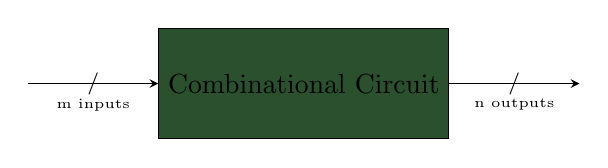
\begin{tikzpicture}[node distance = 3.5cm]
	\node [input] (input) {};
	\node [blockg, right of = input] (block1) {Combinational Circuit};
	\node [output, right of = block1] (output) {};
	
	\draw[-stealth, buswidth={m inputs}] (input) -- (block1);
	\draw[-stealth, buswidth={n outputs}] (block1) -- (output);
\end{tikzpicture} \end{center}

\section{THE BINARY ADDER}

A \keyword{binary adder} performs the addition of bits. In order to construct this circuit, lets first start by creating the truth table. Consider two addition bits x and y, with result r and a carry bit c.
\[
\begin{array}{|c c|c c|}
	\hline
	x & y & r & c \\
	\hline
	0 & 0 & 0 & 0 \\
	0 & 1 & 1 & 0 \\
	1 & 0 & 1 & 0 \\ 
	1 & 1 & 0 & 1 \\
	\hline
\end{array} \]

Using the truth table, we can construct a circuit. This circuit is called a \keyword{half-adder} as it doesnt consider a carry-in bit, and its circuit looks like this.
\\

\begin{center} \begin{circuitikz}
		\draw (2,0) node[and port] (A){};
		\draw (2,-2) node[xor port] (X){};
		\draw (A.in 1) to[short, -*] ++(-3,0) node[label=left:$x$] (x){};
		\draw (A.in 2) to[short, -*] ++(-3,0) node[label=left:$y$] (y){};
		\draw (x) ++(1.5,0) node[circ]{} |- (X.in 1);
		\draw (y) ++(1,0) node[circ]{} |- (X.in 2);
		\draw (A.out) to[short, -*] ++(2,0) node[label=right:$c$] (c){};
		\draw (X.out) to[short, -*] ++(2,0) node[label=right:$r$] (r){};
\end{circuitikz} \end{center}
\vspace{1em}
Suppose we did want to consider a carry in bit. The resulting truth table with the addition of the carry in bit b looks like this. This circuit is called a \keyword{full adder}.

\[
\begin{array}{|c c c|c c|}
	\hline
	x & y & b & r & c \\
	\hline
0                     & 0                     & 0                     & 0                     & 0                     \\
0                     & 0                     & 1                     & 1                     & 0                     \\
0                     & 1                     & 0                     & 1                     & 0                     \\
0                     & 1                     & 1                     & 0                     &  1                     \\
\hline
1                     & 0                     & 0                     & 1                     & 0                     \\
1                     & 0                     & 1                     & 0                     & 1                     \\
1                     & 1                     & 0                     & 0                     & 1                     \\
1                     & 1                     & 1                     & 1                     & 1     \\
	\hline
\end{array} \]

Constructing this circuit directly from the truth table is trivial, but another way to construct a full-adder involves using two half adders. \\

\begin{center} \begin{circuitikz}
		\draw (2,0) node[flipflop HA] (HA1) {HA};
		\draw (5,-3) node[flipflop HA] (HA2) {HA};
		\draw (HA2.pin 4) to ++(1,0) node[or port, anchor=in 2] (OR) {};
		\draw (HA2.pin 1) to[short] ++(-5,0) node[label=left:$c_\text{ in}$, circ]{};
		\draw (HA1.pin 1) to ++(-2,0) node[label=left:$x$, circ]{};
		\draw (HA1.pin 3) to ++(-2,0) node[label=left:$y$, circ]{};
		\draw (HA1.pin 6) to ++(0.5,0) |- (HA2.pin 3);
		\draw (HA1.pin 4) to ++(3.5,0) |- (OR.in 1);
		\draw (OR.out) to ++(1,0) node[label=right:$c_\text{ out}$, circ]{};
		\draw (HA2.pin 6) to ++(4,0) node[label=right:$r$, circ]{};
\end{circuitikz} \end{center}
\vspace{1em}
Now that we have constructed a basic full-adder, we can chain these together to create an arbitrary $n$-bit adder. Below is a 2-bit adder to show how we can extend this concept further to larger sizes (also to avoid drawing a crazy circuit in \TeX)


\part{THE VERILOG HDL}

\chapter{THE BASICS}

\section{HARDWARE DESCRIPTION LANGUAGES}

\keyword{Hardware Description Languages (HDLs)} are a specialized computer language that are used to describe the structure and behavior of \keyword{electronic circuits}, they also include the notion of \keyword{time-delays} present in real digital circuits, and they also support multiple things happening at the same time - \keyword{concurrency}. This is different from programming languages which are line-by-line (sequential) in nature

This document goes over the \keyword{Verilog} HDL which is ubiquitous in the industry, and uses the \texttt{.v} file extension. Another key thing is that HDLs are used \textit{after} designing the hardware, remember that they are NOT programming languages.

\section{LEVELS OF ABSTRACTION}

Within this field of study we commonly encounter the need to use predesigned elements such as registers and multiplexers within more complex designs. When this arises we add a block for the multiplexer, its inputs, and its outputs, and treat it as a block without worrying about how it works. This is called \keyword{abstraction}.

There are three main levels of abstraction provided by Verilog, and we can code things at each level.
\begin{itemize}
	\item Gate Level
	\item Dataflow Level (Register Transfer Level)
	\item Behavioural Level
\end{itemize}

\emph{Gate Level Modeling} allows us to connect hardware gate-by-gate, and wire-by-wire. Verilog has the basic gates ready for use through basic syntax. It is the lowest level of abstraction

\begin{lstlisting}[caption={Basic Gate Level Modeling},label={lst1}]
and G1(out1, A, B);
or G2(out2, A, B);
nand G3(out3, A, B);
\end{lstlisting}

\emph{Register Transfer Level Modeling} allows us to talk about how the data flows in a circuit and it deals with the concept of \keyword{continuous assignment}.

\begin{lstlisting}[caption={Basic RTL Modeling}, label={lst2}]
assign out1 = x & y;
assign out2 = x | y;
assign out3 = ~y;
\end{lstlisting}

\emph{Behavioral Modeling} allows us to describe the behavior of circuits in (almost) plain English, this is the highest level of abstraction and uses keywords such as \code{always} and \code{initial}. It is also usually the fastest way to write simple things such as conditional statements.

\begin{lstlisting}[caption={Basic Behavioral Modeling}, label={lst3}]
always @(sel, I0, I1):
begin
	if (sel)
		out = I1;
	else
		out = I0;
end
\end{lstlisting}

\section{MODULES \& ENTITIES}

A \keyword{module} is the basic building block of Verilog and it can be an element or collection of other lower-level modules. They provide their functionality to higher-level blocks through means of their \keyword{ports}, but they hide the internal implementation. This is essentially the concept of abstraction we discussed earlier, but this also allows for procedural based design. 

\begin{lstlisting}[caption={Module Declaration Syntax}, label={lst4}]
module <moduleName> (
	[port-list]
);
// Module functionality goes here
endmodule
\end{lstlisting}

Aside from declaring modules, we can also create \keyword{entities} by instantiating modules. To learn by example we can use the code for a 2x1 MUX in Snippet \ref{lst3} to create  4x1 MUX.

\begin{lstlisting}[caption={Module Instantition Example (4x1 MUX)}]
// Create the 2x1 MUX module
module mux_2x1 (
	input i0, i1, sel
	output out
);
	always @(i0, i1, sel)
	begin
		if (sel)
			out = i1;
		else
			out = i0;
	end
endmodule

// Create the 4x1 MUX module
module mux_4x1(
	input i0, i1, i2, i3, sel0, sel1,
	output out
);

	wire outA, outB;
	
	2x1mux A (i0,i1,sel0, outA);
	2x1mux B (i2,i3,sel0, outB);
	2x1mux C (outA, outB, sel1, out);
	
endmodule
\end{lstlisting}

\end{document}